\begin{center}
\begin{tikzpicture}
\begin{axis}[
    width=\dimexpr0.5\linewidth-1cm\relax,
    height=\dimexpr0.5\linewidth-1cm\relax,
    grid=both,
    unbounded coords=jump,
    title style={font=\small, yshift=0.6em},
    xlabel=$t$,
    ylabel style={%
        rotate=-90,
        anchor=east,
        overlay%
    },
    ylabel={$\varphi(t)=\dfrac12\ln\Bigl(\dfrac{1-t}{t+1}\Bigr)$},
    xmin=-1.2, xmax=1.2,
    ymin=-2.2, ymax=2.2,
]
\addplot[dashed,gray,samples=2] coordinates {(-1,-4) (-1,4)};
\addplot[dashed,gray,samples=2] coordinates {(1,-4) (1,4)};
\addplot[red,thick,domain=-0.99:0.99,samples=300,restrict y to domain=-4:4]
  {0.5*ln((1-x)/(x+1))};
\addplot[only marks, mark=*, mark size=1.5pt, red] coordinates {(0,0)};
\node[red] at (axis cs:0.15,0.3) {$(0,0)$};
\end{axis}
\end{tikzpicture}
\end{center}